\documentclass{standalone}
\usepackage{fontspec}
\setsansfont{DejaVuSans.ttf}[Path=./,Kerning=Off,Ligatures={TeXOff,NoCommon}]
\usepackage{tikz}
\begin{document}
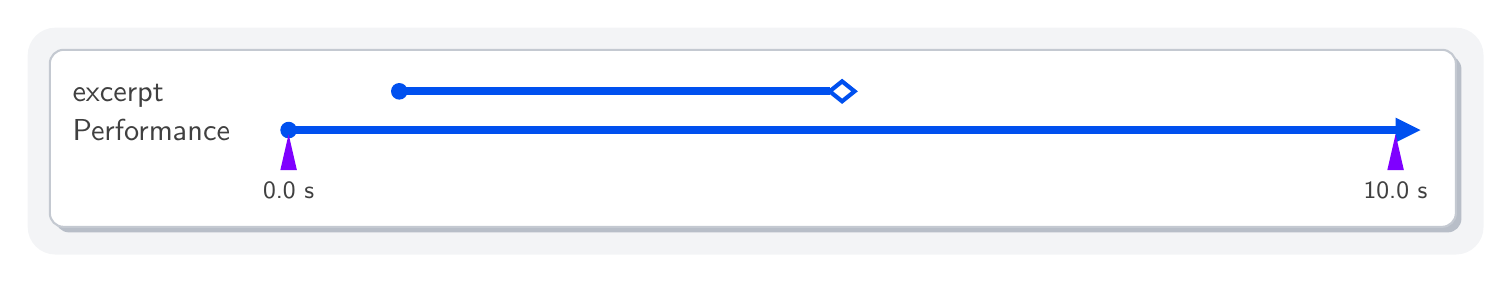
\begin{tikzpicture}[x=1pt,y=1pt,miter limit=4,font=\sffamily]
\definecolor{ts0050EF}{HTML}{0050EF}
\definecolor{ts404040}{HTML}{404040}
\definecolor{ts7F00FF}{HTML}{7F00FF}
\definecolor{tsB8BEC8}{HTML}{B8BEC8}
\definecolor{tsC4C9D1}{HTML}{C4C9D1}
\definecolor{tsF3F4F6}{HTML}{F3F4F6}
\definecolor{tsFFFFFF}{HTML}{FFFFFF}
\begin{scope}[shift={(16,16)}]
\path[rounded corners=10pt,fill=tsF3F4F6] (0,0) rectangle (526.0859,81.9766);
\path[rounded corners=5pt,fill=tsB8BEC8] (10,8) rectangle (518.0859,71.9766);
\path[rounded corners=5pt,fill=tsFFFFFF,draw=tsC4C9D1,line width=0.75pt] (8,10) rectangle (516.0859,73.9766);
\path[draw=ts0050EF,line width=3pt] (94.2915,44.9766) -- (494.2915,44.9766);
\path[fill=ts0050EF] (94.2915,44.9766) circle[radius=3];
\path[fill=ts0050EF] (503.2915,44.9766) -- (494.2915,49.4766) -- (494.2915,40.4766) -- cycle;
\path[draw=ts0050EF,line width=3pt] (134.2915,58.9766) -- (289.7915,58.9766);
\path[fill=ts0050EF] (134.2915,58.9766) circle[radius=3];
\path[draw=ts0050EF,line width=1.5pt] (289.7915,58.9766) -- (294.2915,62.5766) -- (298.7915,58.9766) -- (294.2915,55.3766) -- cycle;
\path[fill=ts7F00FF] (94.2915,43.4766) -- (91.2915,30.4766) -- (97.2915,30.4766) -- cycle;
\path[fill=ts7F00FF] (494.2915,43.4766) -- (491.2915,30.4766) -- (497.2915,30.4766) -- cycle;
\node[anchor=base west,inner sep=0,font=\sffamily\fontsize{11}{12.8047}\selectfont,text=ts404040] at (16,55.1685) {excerpt};
\node[anchor=base west,inner sep=0,font=\sffamily\fontsize{11}{12.8047}\selectfont,text=ts404040] at (16,41.1685) {Performance};
\node[anchor=base,inner sep=0,font=\sffamily\fontsize{9}{10.4766}\selectfont,text=ts404040] at (94.2915,20.1226) {0.0 s};
\node[anchor=base,inner sep=0,font=\sffamily\fontsize{9}{10.4766}\selectfont,text=ts404040] at (494.2915,20.1226) {10.0 s};
\end{scope}
\end{tikzpicture}
\end{document}
